\documentclass[12pt, letterpaper,fleqn]{article}
\usepackage[utf8]{inputenc}
\usepackage{mathtools}
\usepackage{indentfirst}
\usepackage{hyperref}
\usepackage{pgfplots}
\usepackage{listings}
\pgfplotsset{compat=1.9, width=10cm}

\usepgfplotslibrary{external}
\tikzexternalize

\DeclarePairedDelimiter\abs{\lvert}{\rvert}%

\title{Trabalho Prático 3}
\author{Hugo Silva, José Torres}
\date{novembro 2022}

\begin{document}

\maketitle

\section*{Introdução}

Visamos estudar métodos de aproximação numéricos para o cálculo de valores exatos de $f(x)$, sendo $f$ a função em questão.

Durante este trabalho iremos usufruir de \textbf{métodos de interpolação} de funções e usufruiremos também de \textbf{métodos de construção de splines} (maioritariamente cúbicas) para tais funções. 

\section*{Exercício 1}

A função a ser estudade é $f(x) = x^2 + \sin(6x)$ para $x \in \mathopen[-1,1\mathclose]$

\begin{quote}
\centering
    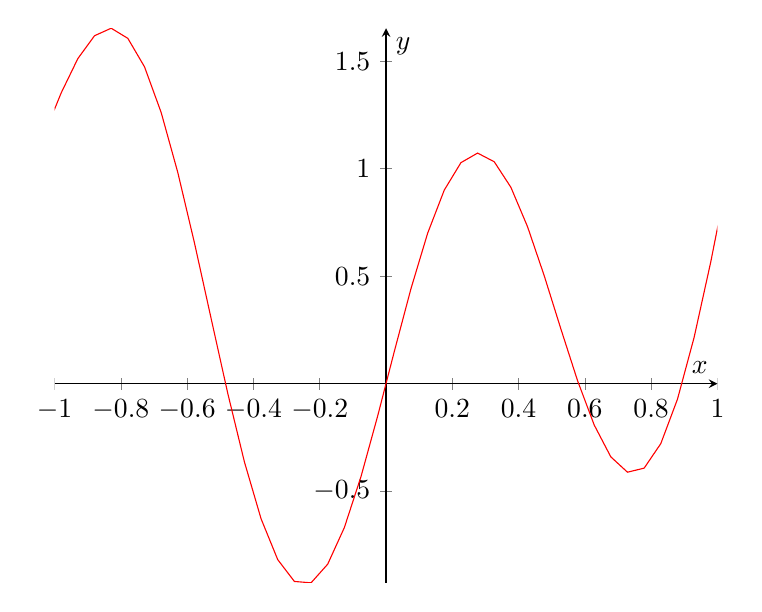
\begin{tikzpicture}
        \begin{axis} [xmin=-1, xmax=1, axis lines=middle, xlabel=$x$, ylabel=$y$]
            \addplot[color=red, samples=200]{x^2 + sin(deg(6*x))};
        \end{axis}
    \end{tikzpicture}
\end{quote}

\begin{itemize}
    \item Pretende-se calcular um conjunto $n+1 = 8$ pontos, ($x_i, f_i = f(x_i)$) inicialmente. \\
    
    Para tal, calculamos atribui-se $x_0 = -1$ e $x_7 = 1$ e, consequentemente, todos os pontos intermédios irão estar divididos em parcelas aproximadamente iguais entre $x_0 e x_7$, parcelas essas que podem ser calculadas através da amplitude $h$:

    \[h = \frac{b-a}{n}\]

    Onde $\mathopen[-1,1\mathclose] = \mathopen[a,b\mathclose]$ e $n = 7$. \\
    
    Da fórmula acima indicada temos o desenvolvimento:

    \[h = \frac{1-(-1)}{7} = \frac{2}{7} \approx 0.286\]

    E finalmente temos que:

    \[x_n = x_0 + h\times n \Leftrightarrow x_n = -1 + 0.286n\]

    Por fim obtemos a tabela de valores:
    
    \begin{center}
        \begin{tabular} {|| c | c | c | c | c | c | c | c | c ||} \hline
            $i$ & $0$ & $1$ & $2$ & $3$ & $4$ & $5$ & $6$ & $7$\\ [0.4ex]\hline
            $x_i$ & $-1$ & $-0.714$ & $-0.428$ & $-0.142$ & $0.144$ & $0.430$ & $0.716$ & $1$ \\ [0.4ex]\hline
        \end{tabular}
    \end{center}

    \textbf{\textit{NOTA:}} Os valores de $x_i$ são arredondados devido ao facto da amplitude resultar de um valor aproximado, portanto o intervalo entre $[0.716,1]$ é mais pequeno do que o intervalo entre $[0.430, 0.716]$, porém não é algo que influencie o resultado final de forma avassaladora.

    Por ser suficiente manteve-se os intervalos representados por apenas 3 casas decimais.

    \item \textbf{\textit{Interpolação por método de Newton}} - Tendo a tabela de valores de $x_i$ disponíveis, é possível aplicar os métodos de aproximação numérica a $f(x)$.

    Comecemos pelo método de interpolação. Foi feita a escolha de usar o método de interpolação de Newton, visto que é um método mais simples para gerar o polinómio que descreve a interpolação. Em questão de geração e escrita de código, este método é um pouco mais complexo do que o método de Lagrange, visto que o método de Newton é descrito pela equação:

    \[p_n(x) = f(x_0) + (x-x_0)f[x_0,x_1] + ... + (x-x_0)...(x-x_{n-1})f[x_0, ... , x_n]\]

    O cálculo das diferenças divididas $f[x_0, ... , x_n]$ acaba por ser mais complexo algoriticamente do que a fórmula dada pelo método de Lagrange. \\
    
    Sabe-se também que uma diferença dividida de $f[x_k, ... , x_n]$ é dada pela equação:

    \[f[x_k, ... , x_n] = \frac{f[x_{k+1}, ... , x_n] - f[x_k, ..., x_{n-1}]}{x_n - x_k}\]

    Vindo de um background computacional, o grupo decidiu representar as diferenças divididas numa matrix $n\times n$.

    Suponhamos que possuímos então uma matrix $M$, onde o valor da diferença dividida numa linha $I$ e numa coluna $J$ é dada por $M[I][J]$.
    Sabe-se inicialmente que a primeira linha vai possuir os valores de $f(x_i)$ e que a partir desse ponto podemos aplicar um algoritmo que calcule o resto das diferenças. Tal algoritmo é descrito sob a forma:

    \[M[I][J] = \frac{M[I-1][J+1] - M[I-1][J]}{x_j - x_{i+j}}\]

    Seguindo o algoritmo em cima temos o código gerado:
    \begin{verbatim}
        #define LEN 7
        double m[LEN+1][LEN+1];
        double xn[LEN+1] = {-1, -0.714, -0.428, -0.142, 0.144, 0.430, 
                            0.716, 1};
    
        // f(xi) -> f[x0, ... ,xn]
        void dividedDiff() {
            // preenchimento da 1º linha com valores f(xi)
            for (int i = 0; i <= LEN; i++) {
                m[0][i] = f(xn[i]);
            }
        
            // calculo das restantes diferencas
            int limite = LEN-1; // evitar calculos impossiveis
            for (int i = 1; i <= LEN; i++) {
                for (int j = 0; j <= limite; j++) {
                    m[i][j] = (m[i-1][j+1] - m[i-1][j]) / (xn[j] - xn[i+j]);
                }
                --limite;
            }
        }
    \end{verbatim}

    Para além das diferenças divididas, existe a componente $(x-x_0)...(x-x_n)$ necessária na aplicação do método de interpolação.

    Foi denominada de função $h(x,i)$ a cada componente individual, ou seja, $h(x, 2) = (x-x_2)$:

    \begin{verbatim}
        double xn[LEN+1] = {-1, -0.714, -0.428, -0.142, 0.144, 0.430, 
                            0.716, 1};
                            
        // (x - x0)(x - x1)...(x - xn)
        double h(double x, int i) {
            return x - xn[i];
        }
    \end{verbatim}

    Basta agora aplicar o método de Newton pela definição:

    \begin{verbatim}
        // f(x0) + h(0)f[x0, x1] + ... + h(n-1)f[x0, ... , xn]
        double newton(double x) {
            // var do valor aproximado a ser calculado
            double val = 0;
        
            // var que guarda (x-x0)(x-x1)...(x-xn), etc
            double hval = 1;
        
            // aplicacao da definicao do metodo de Newton
            for (int i = 0; i <= LEN; i++) {
                val += hval*m[i][0];
                hval *= h(x, i);
            }
            
            return val;
        }
    \end{verbatim}

    \textbf{\textit{NOTA:}} Fazendo por matrix os valores de $f[x_0, ... , x_n]$ vão ficar sempre posicionados na primeira coluna ($J=0$) , sendo a razão porque apenas multiplicamos os $hval$ pelos valores $M[I][0]$ e posteriormente somamos a $val$. \\

    Prosseguiu-se ao cálculo de 200 pontos distintos através do algoritmo acima indicado, o que acabou por gerar o seguinte gráfico $g(x)$:

    \begin{quote}
        \centering
        \begin{tikzpicture}
            \begin{axis} [xmin=-1, xmax=1, axis lines=middle, xlabel=$x$, ylabel=$y$]
                \addplot[color=blue]
                table[meta=Y]
                {newtonOut.txt};
            \end{axis}
        \end{tikzpicture}
    \end{quote}

    COMPARACAO COM O F(X) [terminar com o da spline cubica ao lado]

    \begin{quote}
        \centering
        \begin{tikzpicture}
            \begin{axis} [xmin=-1, xmax=1, axis lines=middle, xlabel=$x$, ylabel=$y$]
                \addplot[color=blue]
                table[meta=Y]
                {newtonOut.txt};
                \addplot[color=red, samples=200]{x^2 + sin(deg(6*x))};
            \end{axis}
        \end{tikzpicture}
    \end{quote}
    
    \item \textbf{\textit{Spline Cúbico Natural}} - Para a realização dos exercícios sobre o \textit{spline cúbico natural} foi usada a linguagem Python pelo facto de esta ter bibliotecas simples e mais fáceis de utilizar para a resolução do sistema para encontrar os valores dos multiplicadores (\textit{M_i}).

    $$
    \begin{bmatrix}
    1 & 0 & 0 & 0 & 0 & 0 & 0 & 0 \\[6pt]
    \frac{h}{6} & \frac{2h}{3} & \frac{h}{6} & 0 & 0 & 0 & 0 & 0 \\[6pt]
    0 & \frac{h}{6} & \frac{2h}{3} & \frac{h}{6} & 0 & 0 & 0 & 0 \\[6pt]
    0 & 0 & \frac{h}{6} & \frac{2h}{3} & \frac{h}{6} & 0 & 0 & 0 \\[6pt]
    0 & 0 & 0 & \frac{h}{6} & \frac{2h}{3} & \frac{h}{6} & 0 & 0 \\[6pt]
    0 & 0 & 0 & 0 & \frac{h}{6} & \frac{2h}{3} & \frac{h}{6} & 0 \\[6pt]
    0 & 0 & 0 & 0 & 0 & \frac{h}{6} & \frac{2h}{3} & \frac{h}{6} \\[6pt]
    0 & 0 & 0 & 0 & 0 & 0 & 0 & 1 \\
    \end{bmatrix}
    \cdot 
    \begin{bmatrix}
    M_0 \\[6pt]
    M_1 \\[6pt]
    M_2 \\[6pt]
    M_3 \\[6pt]
    M_4 \\[6pt]
    M_5 \\[6pt]
    M_6 \\[6pt]
    M_7 \\[6pt]
    \end{bmatrix}
    =
    \begin{bmatrix}
    0 \\[6pt] 
    -6.710 \\[6pt]
    4.916  \\[6pt]
    6.596  \\[6pt]
    -5.515 \\[6pt]
    -3.691 \\[6pt]
    7.839  \\[6pt]
    0 \\[6pt]
    \end{bmatrix}
    $$
    Resolvendo este sistema, usando a biblioteca \textit{numpy} e a função \textit{linalg.solve} da linguagem Python, o resultado é:
    \begin{equation}
        M(x)=\begin{cases}
            M_0 = 0.000   \\
            M_1 = -42.025 \\
            M_2 = 27.341  \\
            M_3 = 35.789  \\
            M_4 = -32.111 \\
            M_5 = -23.048 \\
            M_6 = 46.873  \\
            M_7 = 0.000       
        \end{cases}
    \end{equation}
    \textbf{\textit{NOTA:}} Todos os valores são arredondados a três casas decimais, já que a linguagem usada apresenta os resultados com uma precisão de 14 casas decimais.
    
    Usando os resultados do sistema acima e da expressão geral para construção de $S_i(x)$,
    \begin{equation}
    S_i(x) = M_{i-1} \cdot \frac{(x_i - x)^3}{6h_i} + M_i \cdot \frac{(x-x_{i-1})^3}{6h_i}+(f_{i-1} - M_{i-1} \cdot \frac{h_i^2}{6})\cdot \frac{(x_i - x)}{h_i} + (f_i - M_i \cdot \frac{h_i^2}{6})\cdot \frac{(x-x_{i-1})}{h_i}&&
    \end{equation}
    obtém-se a seguinte equação do spline cúbico natural:
    \begin{equation}
        S(x) = \begin{cases}
            M_0\frac{(x_1 - x)^3}{6h} + M_1\frac{(x-x_0)^3}{6h}+(f_0 - M_0\frac{h^2}{6})\frac{(x_1 - x)}{h} + (f_1 - M_1\frac{h^2}{6}) \frac{(x-x_0)}{h}, & x_0 \leq x \leq x_1 \\
            
            M_1\frac{(x_2 - x)^3}{6h} + M_2\frac{(x-x_1)^3}{6h}+(f_1 - M_1\frac{h^2}{6})\frac{(x_2 - x)}{h} + (f_2 - M_2\frac{h^2}{6}) \frac{(x-x_1)}{h}, & x_1 \leq x \leq x_2 \\
            
            M_2\frac{(x_3 - x)^3}{6h} + M_3\frac{(x-x_2)^3}{6h}+(f_2 - M_2\frac{h^2}{6})\frac{(x_3 - x)}{h} + (f_3 - M_3\frac{h^2}{6}) \frac{(x-x_2)}{h}, & x_2 \leq x \leq x_3 \\
            
            M_3\frac{(x_4 - x)^3}{6h} + M_4\frac{(x-x_3)^3}{6h}+(f_3 - M_3\frac{h^2}{6})\frac{(x_4 - x)}{h} + (f_4 - M_4\frac{h^2}{6}) \frac{(x-x_3)}{h}, & x_3 \leq x \leq x_4 \\

            M_4\frac{(x_5 - x)^3}{6h} + M_5\frac{(x-x_4)^3}{6h}+(f_4 - M_4\frac{h^2}{6})\frac{(x_5 - x)}{h} + (f_5 - M_5\frac{h^2}{6}) \frac{(x-x_4)}{h}, & x_4 \leq x \leq x_5 \\
            
            M_5\frac{(x_6 - x)^3}{6h} + M_6\frac{(x-x_5)^3}{6h}+(f_5 - M_5\frac{h^2}{6})\frac{(x_6 - x)}{h} + (f_6 - M_6\frac{h^2}{6}) \frac{(x-x_5)}{h}, & x_5 \leq x \leq x_6 \\
            
            M_6\frac{(x_7 - x)^3}{6h} + M_7\frac{(x-x_6)^3}{6h}+(f_6 - M_6\frac{h^2}{6})\frac{(x_7 - x)}{h} + (f_7 - M_7\frac{h^2}{6}) \frac{(x-x_6)}{h}, & x_6 \leq x \leq x_7 \\
        \end{cases}    
    \end{equation}
    \textbf{\textit{NOTA:}} Optou-se por não se substituir as variáveis e constantes no sistema acima pelos respetivos valores por uma questão de formatação.
    
    O código utilizador para a construção do spline foi o seguinte:
    \begin{verbatim}
        import numpy as np
        import matplotlib.pyplot as plt 
        n = 7, h = 0.286
        # Abcissas
        xn = [-1.000, -0.714, -0.428, -0.142, 0.144, 0.430, 0.716, 1.000]
        
        # Função f(x) = x² + sin(6x)
        def f(x):
            return x**2 + (np.sin(6*x))
        # Cálculo dos valores de f(xi)
        fi = []
        for i in range(n+1):
            fi += [f(xn[i]]
        
        # Função Spline
        def spline(x):
            if xn[0] <= x <= xn[1]:
                return (M[1]*(x-xn[0])**3/(6*h))+(fi[0]*(xn[1]-x)/h) 
                        +((fi[1]-(M[1]*h**2)/6)*(x-xn[0])/h)
            (...)
        # Cálculo do sistema para encontrar os M's
        A = [ [1, 0, 0, 0, 0, 0, 0, 0],
              [h/6, 2*h/3, h/6, 0, 0, 0, 0, 0],
              [0, h/6, 2*h/3, h/6, 0, 0, 0, 0],
              [0, 0, h/6, 2*h/3, h/6, 0, 0, 0],
              [0, 0, 0, h/6, 2*h/3, h/6, 0, 0],
              [0, 0, 0, 0, h/6, 2*h/3, h/6, 0],
              [0, 0, 0, 0, 0, h/6, 2*h/3, h/6],
              [0, 0, 0, 0, 0, 0, 0, 1]                                
            ]
        B = [0]
        for i in range (1,n):
            B += [ (fi[i+1]-fi[i])/h - (fi[i]-fi[i-1])/h ]
        B += [0]
        M = np.linalg.solve(A,B)
        S = np.vectorize(spline)
        # Gráficos
        x = np.arange(start = -1, stop = 1, step = 0.001)
        y = S(x)
        ff = f(x)
        y2 = erro_spline(x)
        plt.plot(x, ff, label = 'f(x)')
        plt.plot(x, y, 'r-', label = 's(x)')
    \end{verbatim}
    
    O gráfico obtido com o código descrito foi o seguinte:
    \begin{figure}
        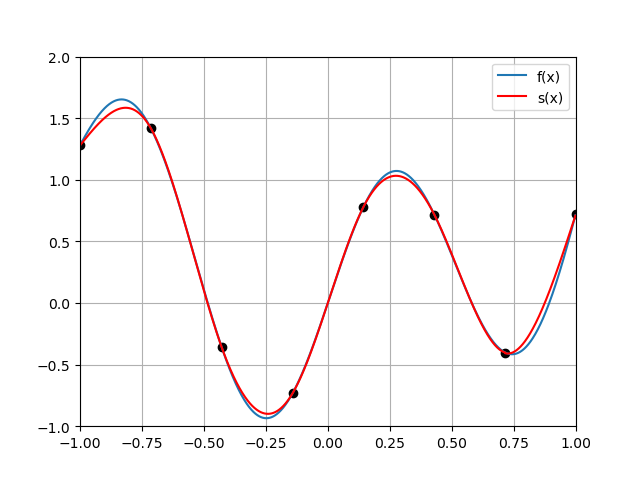
\includegraphics[width=\linewidth]{ex1-spline.png}
        \caption{Spline cúbico natural do conjunto de pontos do exercício 1}
        \label{fig:spline1}
    \end{figure}
    %Figure \ref{fig:spline1} shows a the spline
\end{itemize}


\end{document}


